\chapter{Resultados}
\label{cap:resultados}

Este capítulo apresenta os resultados obtidos pela aplicação da metodologia proposta ao estudo de caso de Mossoró-RN, com foco nos ODS 9 (Indústria, Inovação e Infraestrutura) e ODS 16 (Paz, Justiça e Instituições Eficazes). Os dados foram coletados e analisados utilizando o sistema implementado, conforme descrito no capítulo anterior.

\section{Visão Geral da Coleta}
\label{sec:coleta-geral}

O sistema foi executado com o modelo Gemini 2.5 Flash como provedor principal de análise. A Tabela~\ref{tab:resumo-coleta} apresenta o resumo quantitativo da coleta realizada para os dois ODS.

\begin{table}[h!]
    \centering
    \caption{Resumo quantitativo da coleta de dados por ODS em Mossoró-RN}
    \label{tab:resumo-coleta}
    \begin{tabular}{lcc}
        \hline
        \textbf{Métrica} & \textbf{ODS 9} & \textbf{ODS 16} \\
        \hline
        Total de análises coletadas & 253 & 116 \\
        Estabelecimentos únicos analisados & 117 & 12 \\
        Problemas detectados & 144 & 54 \\
        Percentual de análises com problema & 56,9\% & 46,6\% \\
        Score médio de confiança & 0,87 & 0,84 \\
        \hline
    \end{tabular}
    \legend{Fonte: Elaborado pelo autor (2025).}
\end{table}

\section{ODS 9 -- Indústria, Inovação e Infraestrutura}
\label{sec:resultados-ods9}

\subsection{Distribuição por Tipo de Estabelecimento}
\label{subsec:tipos-ods9}

As 253 análises do ODS 9 foram coletadas em 117 estabelecimentos únicos, abrangendo sete categorias de locais relacionadas às dimensões do objetivo:

\begin{itemize}
    \item \textbf{Infraestrutura de transporte}: rodoviárias, aeroporto, terminais rodoviários, estações e paradas de ônibus;
    \item \textbf{Infraestrutura urbana}: ruas, avenidas, pontes, viadutos, pavimentação e iluminação pública;
    \item \textbf{Tecnologia e telecomunicações}: lojas de eletrônicos, operadoras de telefonia, provedores de internet e serviços de tecnologia;
    \item \textbf{Indústria}: fábricas, parques industriais e empresas de transformação;
    \item \textbf{Energia}: distribuidoras de energia elétrica e serviços de energia renovável;
    \item \textbf{Micro e pequenas empresas}: comércios locais, serviços de apoio ao empreendedorismo e instituições de crédito para pequenos negócios;
    \item \textbf{Inovação}: \textit{startups}, incubadoras e espaços de inovação.
\end{itemize}

Essa diversidade de tipos de local permitiu capturar percepções sobre todas as sete dimensões do ODS 9, desde ativos físicos de infraestrutura até o ambiente de negócios e inovação do município.

\subsection{Distribuição de Sentimentos}
\label{subsec:sentimentos-ods9}

Das 253 análises coletadas para o ODS 9, a distribuição de sentimentos revelou um cenário predominantemente negativo, conforme apresentado na Tabela~\ref{tab:sentimentos-ods9} e na Figura~\ref{fig:sentimentos-comparados}, que compara a distribuição de sentimentos entre os dois ODS analisados.

\begin{table}[h!]
    \centering
    \caption{Distribuição de sentimentos -- ODS 9 (Mossoró-RN)}
    \label{tab:sentimentos-ods9}
    \begin{tabular}{lcc}
        \hline
        \textbf{Sentimento} & \textbf{Quantidade} & \textbf{Percentual} \\
        \hline
        Positivo & 37 & 14,6\% \\
        Negativo & 103 & 40,7\% \\
        Neutro & 113 & 44,7\% \\
        \hline
        \textbf{Total} & \textbf{253} & \textbf{100\%} \\
        Contribuem para baixo ODS 9 & 144 & 56,9\% \\
        \hline
    \end{tabular}
    \legend{Fonte: Elaborado pelo autor (2025).}
\end{table}

\begin{figure}[h!]
    \centering
    \caption{Distribuição de sentimentos por ODS em Mossoró-RN}
    \label{fig:sentimentos-comparados}
    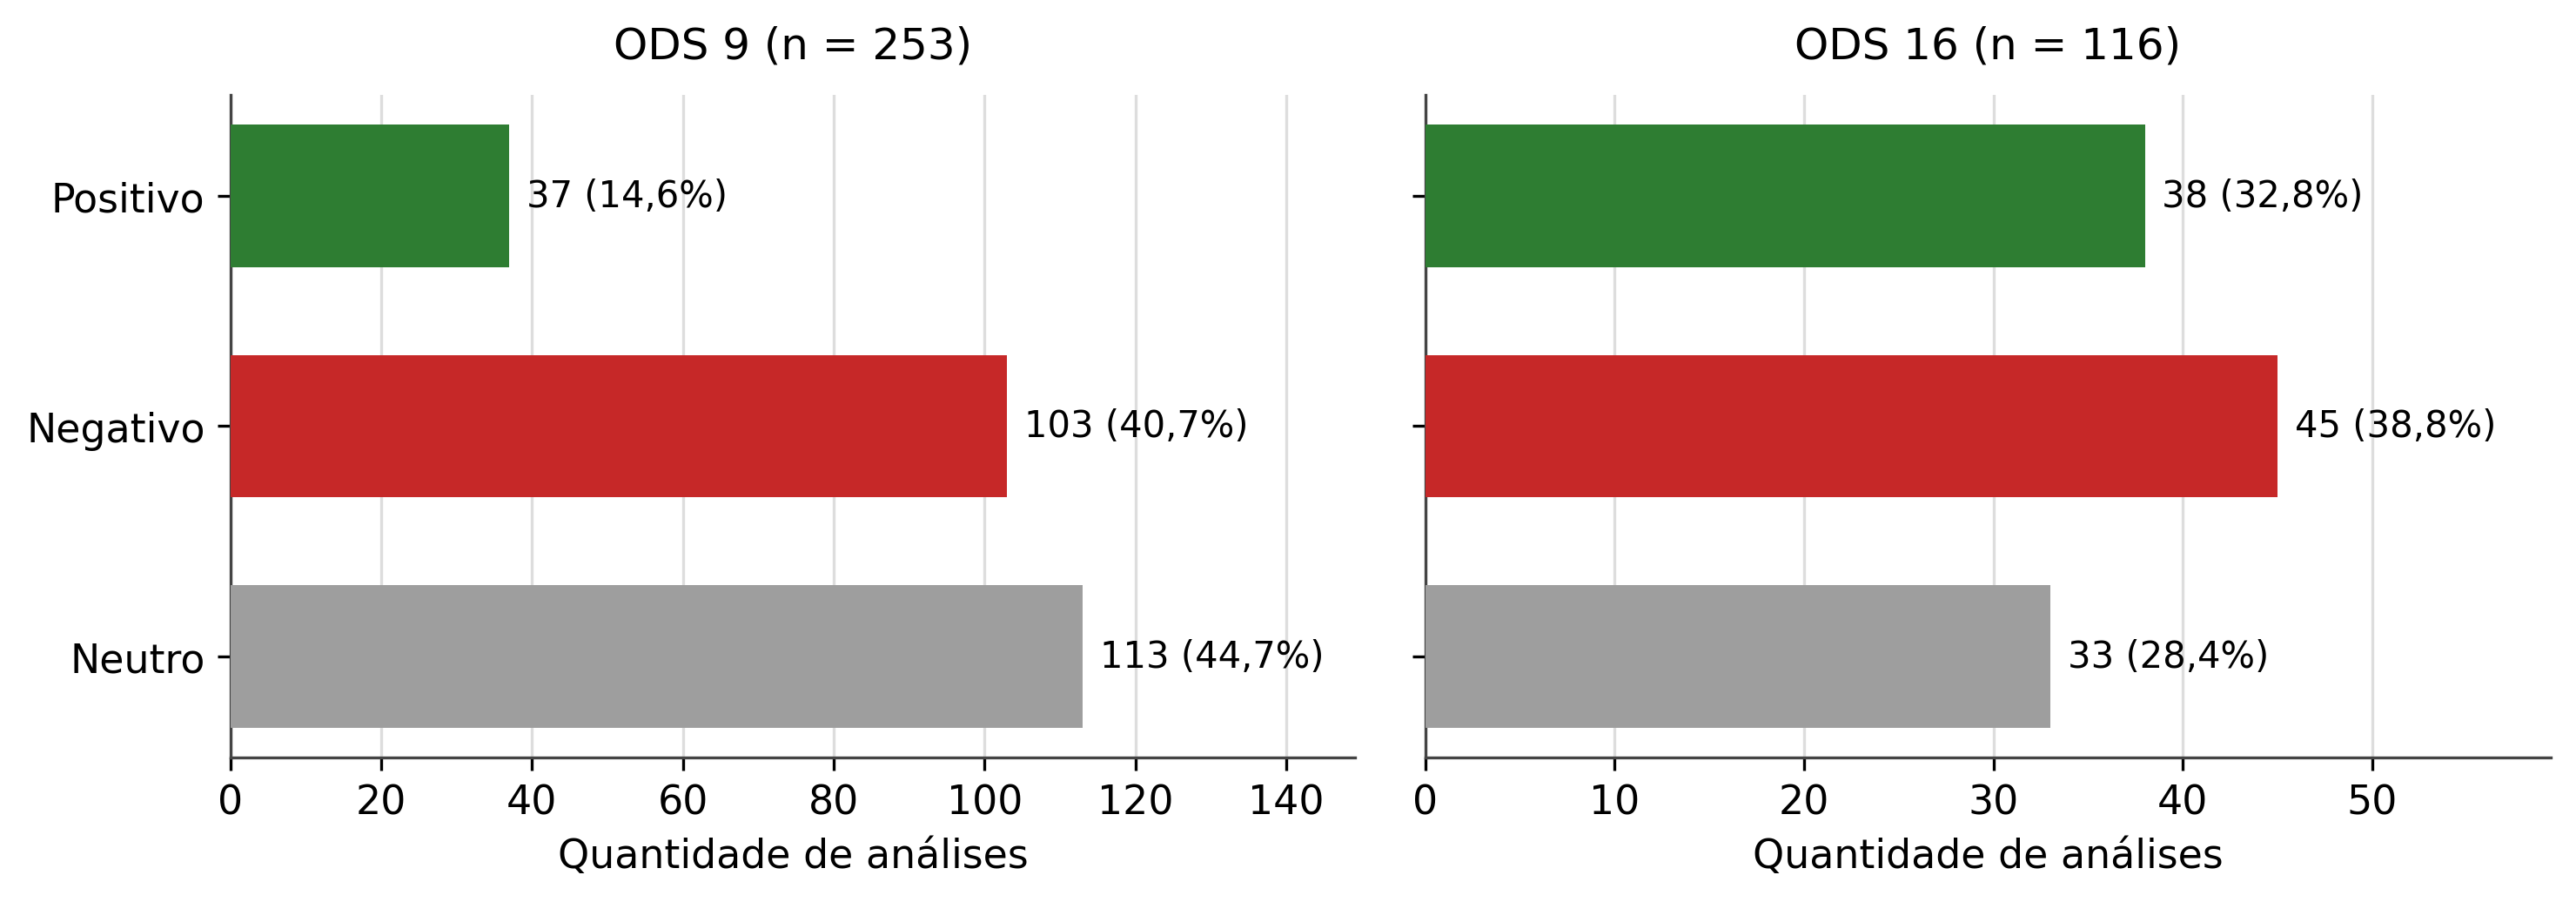
\includegraphics[width=0.95\textwidth]{figuras/distribuicao-sentimentos-ods}
    \legend{Fonte: Elaborado pelo autor (2026).}
\end{figure}

A baixa proporção de avaliações positivas (14,6\%) e o fato de que 56,9\% das análises contribuem diretamente para o baixo desempenho validam a pontuação muito baixa (0--39,99) atribuída a Mossoró no ODS 9 pelo IDSC \cite{idsc2024}. Os scores de confiança elevados (média de 0,87) indicam que o modelo identificou com segurança os aspectos problemáticos nos textos analisados.

A elevada taxa de comentários neutros (44,7\%) pode ser interpretada de duas formas complementares: por um lado, pode indicar relatos descritivos com baixo conteúdo avaliativo explícito; por outro, pode refletir uma normalização de problemas crônicos, em que deficiências recorrentes passam a ser percebidas como parte do cotidiano urbano. Essa leitura reforça a importância da análise por aspecto, uma vez que avaliações aparentemente neutras podem, ao serem analisadas semanticamente, revelar indícios de problemas persistentes.

\subsection{Distribuição de Problemas por Dimensão}
\label{subsec:problemas-ods9}

A Tabela~\ref{tab:problemas-ods9} apresenta a distribuição quantitativa de menções problemáticas por dimensão do ODS 9, extraída do campo de aspectos problemáticos identificados pela IA em cada análise.

\begin{table}[h!]
    \centering
    \caption{Distribuição de menções problemáticas por dimensão -- ODS 9 (Mossoró-RN)}
    \label{tab:problemas-ods9}
    \begin{tabular}{lcc}
        \hline
        \textbf{Dimensão} & \textbf{Menções} & \textbf{Percentual} \\
        \hline
        Infraestrutura Resiliente e Moderna & 85 & 33,6\% \\
        Transporte Público e Mobilidade & 54 & 21,3\% \\
        Acesso à Tecnologia e Informação & 52 & 20,6\% \\
        Valorização da Micro e Pequena Empresa & 48 & 19,0\% \\
        Industrialização Inclusiva e Sustentável & 37 & 14,6\% \\
        Inovação e Pesquisa & 30 & 11,9\% \\
        Eficiência Energética & 29 & 11,5\% \\
        \hline
    \end{tabular}
    \legend{Fonte: Elaborado pelo autor (2026). Percentuais calculados sobre as 253 análises; uma mesma análise pode mencionar problemas em mais de uma dimensão.}
\end{table}

A distribuição evidencia que os problemas do ODS 9 em Mossoró concentram-se nas dimensões físicas e econômicas de base, detalhadas a seguir:

\textbf{Infraestrutura Resiliente e Moderna (85 menções -- 33,6\%)}: dimensão mais problemática do conjunto. O Terminal Rodoviário de Mossoró emergiu como o principal foco de problemas: as avaliações descrevem um equipamento em estado crítico de deterioração, com estruturas abandonadas, risco de queda, condições insalubres (banheiros imundos, ausência de limpeza), iluminação inadequada e falta de manutenção preventiva. A totalidade dos comentários sobre o terminal classificou a infraestrutura como negativa, com scores de confiança acima de 0,85.

\textbf{Transporte Público e Mobilidade (54 menções -- 21,3\%)}: as avaliações do terminal rodoviário e de paradas de ônibus apontam para um sistema de transporte público em colapso: ausência de serviços básicos essenciais, falta de controle sanitário, experiência do usuário altamente comprometida e conectividade regional prejudicada.

\textbf{Acesso à Tecnologia e Informação (52 menções -- 20,6\%)}: as queixas concentram-se em operadoras de telefonia e provedores de internet, com relatos de instabilidade do serviço, atendimento deficiente e cobertura desigual entre regiões da cidade.

\textbf{Valorização da Micro e Pequena Empresa (48 menções -- 19,0\%)}: as análises revelam ausência de comércios básicos em locais estratégicos, limitadas oportunidades para pequenos negócios e insuficiência de suporte ao empreendedorismo local. É a dimensão com maior número absoluto de menções nas avaliações (171 análises a mencionam), refletindo o peso do comércio local na amostra.

As dimensões de Industrialização (14,6\%), Inovação e Pesquisa (11,9\%) e Eficiência Energética (11,5\%) apresentaram menor volume de menções problemáticas, em parte pela menor presença desses tipos de estabelecimento na amostra coletada. Em termos de localização, os estabelecimentos com maior concentração de análises problemáticas foram a Rodoviária de Mossoró, o Terminal Rodoviário Diram Ramos do Amaral, o Aeroporto Dix-Sept Rosado e a Secretaria Municipal de Infraestrutura, Meio Ambiente, Urbanismo e Serviços Urbanos, reforçando o padrão de concentração de problemas em equipamentos de transporte e órgãos de gestão urbana.

\subsection{Dashboard ODS 9}
\label{subsec:dashboard-ods9}

A Figura~\ref{fig:dashboard-ods9} apresenta o dashboard web desenvolvido para visualização dos resultados do ODS 9. A interface substitui a abordagem inicialmente prevista em Microsoft Power BI por uma solução HTML, CSS e JavaScript, acessível diretamente pelo navegador.

\begin{figure}[h!]
    \centering
    \caption{Dashboard web -- ODS 9: Indústria, Inovação e Infraestrutura em Mossoró-RN}
    \label{fig:dashboard-ods9}
    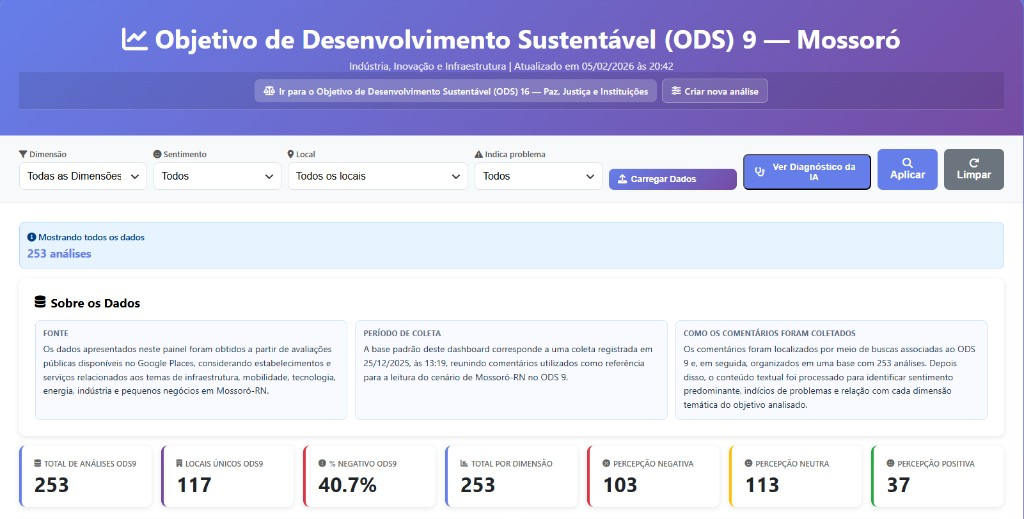
\includegraphics[width=0.95\textwidth]{figuras/dashboard-web-ods9}
    \legend{Fonte: Elaborado pelo autor (2025).}
\end{figure}

O dashboard possibilita filtragem dinâmica por dimensão, sentimento, local e indicação de problema, além da visualização de métricas consolidadas, cards informativos e acesso direto ao diagnóstico gerado pela IA. Essa organização facilita a leitura dos resultados por gestores públicos e especialistas, sem exigir conhecimento prévio em ferramentas proprietárias de inteligência de negócios.

\section{ODS 16 -- Paz, Justiça e Instituições Eficazes}
\label{sec:resultados-ods16}

\subsection{Composição da Amostra}
\label{subsec:amostra-ods16}

Para o ODS 16, foram coletadas 116 análises válidas distribuídas entre 12 estabelecimentos únicos. Embora aparentemente pequena, essa amostra representa os principais órgãos de justiça e segurança pública de Mossoró-RN, incluindo:

\begin{itemize}
    \item \textbf{Órgãos de segurança pública}: delegacias, polícia militar, guarda civil municipal e batalhões;
    \item \textbf{Poder judiciário}: fóruns, tribunais, defensoria pública e Ministério Público;
    \item \textbf{Instituições públicas}: prefeitura, secretarias municipais e câmara municipal;
    \item \textbf{Órgãos eleitorais}: TRE e Justiça Eleitoral;
    \item \textbf{Espaços públicos}: praças e parques, quando as avaliações mencionam segurança ou insegurança.
\end{itemize}

A amostra de 12 estabelecimentos reflete a realidade institucional do município: Mossoró possui um número limitado de órgãos públicos de justiça e segurança formalmente cadastrados na Google Places API, e o sistema capturou os principais estabelecimentos disponíveis. Essa cobertura dos órgãos institucionais relevantes garante que as análises representem adequadamente as percepções sobre o ODS 16 na cidade, ainda que o número absoluto de locais seja menor do que o do ODS 9, que inclui também estabelecimentos comerciais e de infraestrutura.

\subsection{Distribuição de Sentimentos}
\label{subsec:sentimentos-ods16}

A distribuição de sentimentos revela um padrão polarizado, conforme a Tabela~\ref{tab:sentimentos-ods16}. A comparação com o ODS 9, apresentada na Figura~\ref{fig:sentimentos-comparados}, evidencia diferenças relevantes no padrão de avaliação: enquanto o ODS 9 é dominado por avaliações neutras e negativas, o ODS 16 apresenta maior proporção de avaliações positivas, convivendo com queixas concentradas em dimensões críticas.

\begin{table}[h!]
    \centering
    \caption{Distribuição de sentimentos -- ODS 16 (Mossoró-RN)}
    \label{tab:sentimentos-ods16}
    \begin{tabular}{lcc}
        \hline
        \textbf{Sentimento} & \textbf{Quantidade} & \textbf{Percentual} \\
        \hline
        Positivo & 38 & 32,8\% \\
        Negativo & 45 & 38,8\% \\
        Neutro & 33 & 28,4\% \\
        \hline
        \textbf{Total} & \textbf{116} & \textbf{100\%} \\
        Contribuem para baixo ODS 16 & 54 & 46,6\% \\
        \hline
    \end{tabular}
    \legend{Fonte: Elaborado pelo autor (2025).}
\end{table}

Embora a proporção de avaliações positivas (32,8\%) seja maior do que no ODS 9, a concentração de problemas em dimensões críticas -- especialmente instituições eficazes (37,1\% das análises) e segurança pública (11,2\%) -- é suficiente para manter a pontuação na faixa muito baixa. Esse resultado é coerente com a natureza do ODS 16, no qual a experiência do cidadão é influenciada pela qualidade do atendimento, pela eficiência administrativa e pela transparência dos processos, elementos que tendem a gerar avaliações mais emocionalmente carregadas do que as associadas a infraestruturas físicas.

\subsection{Distribuição de Problemas por Dimensão}
\label{subsec:dimensoes-ods16}

A Tabela~\ref{tab:problemas-ods16} apresenta a distribuição quantitativa de menções de problemas por dimensão do ODS 16, e a Figura~\ref{fig:problemas-dimensao-ods16} evidencia graficamente a assimetria entre a dimensão dominante e as demais.

\begin{table}[h!]
    \centering
    \caption{Distribuição de problemas por dimensão -- ODS 16 (Mossoró-RN)}
    \label{tab:problemas-ods16}
    \begin{tabular}{lcc}
        \hline
        \textbf{Dimensão} & \textbf{Menções} & \textbf{Percentual} \\
        \hline
        Instituições Eficazes e Responsáveis & 43 & 37,1\% \\
        Direitos Humanos e Estado de Direito & 14 & 12,1\% \\
        Segurança Pública e Redução da Violência & 13 & 11,2\% \\
        Acesso à Justiça & 12 & 10,3\% \\
        Transparência e Combate à Corrupção & 8 & 6,9\% \\
        Participação Cidadã e Accountability & 6 & 5,2\% \\
        Proteção de Crianças e Grupos Vulneráveis & 6 & 5,2\% \\
        \hline
    \end{tabular}
    \legend{Fonte: Elaborado pelo autor (2025). Percentuais calculados sobre as 116 análises; uma mesma análise pode mencionar problemas em mais de uma dimensão.}
\end{table}

\begin{figure}[h!]
    \centering
    \caption{Distribuição de problemas por dimensão -- ODS 16 (Mossoró-RN)}
    \label{fig:problemas-dimensao-ods16}
    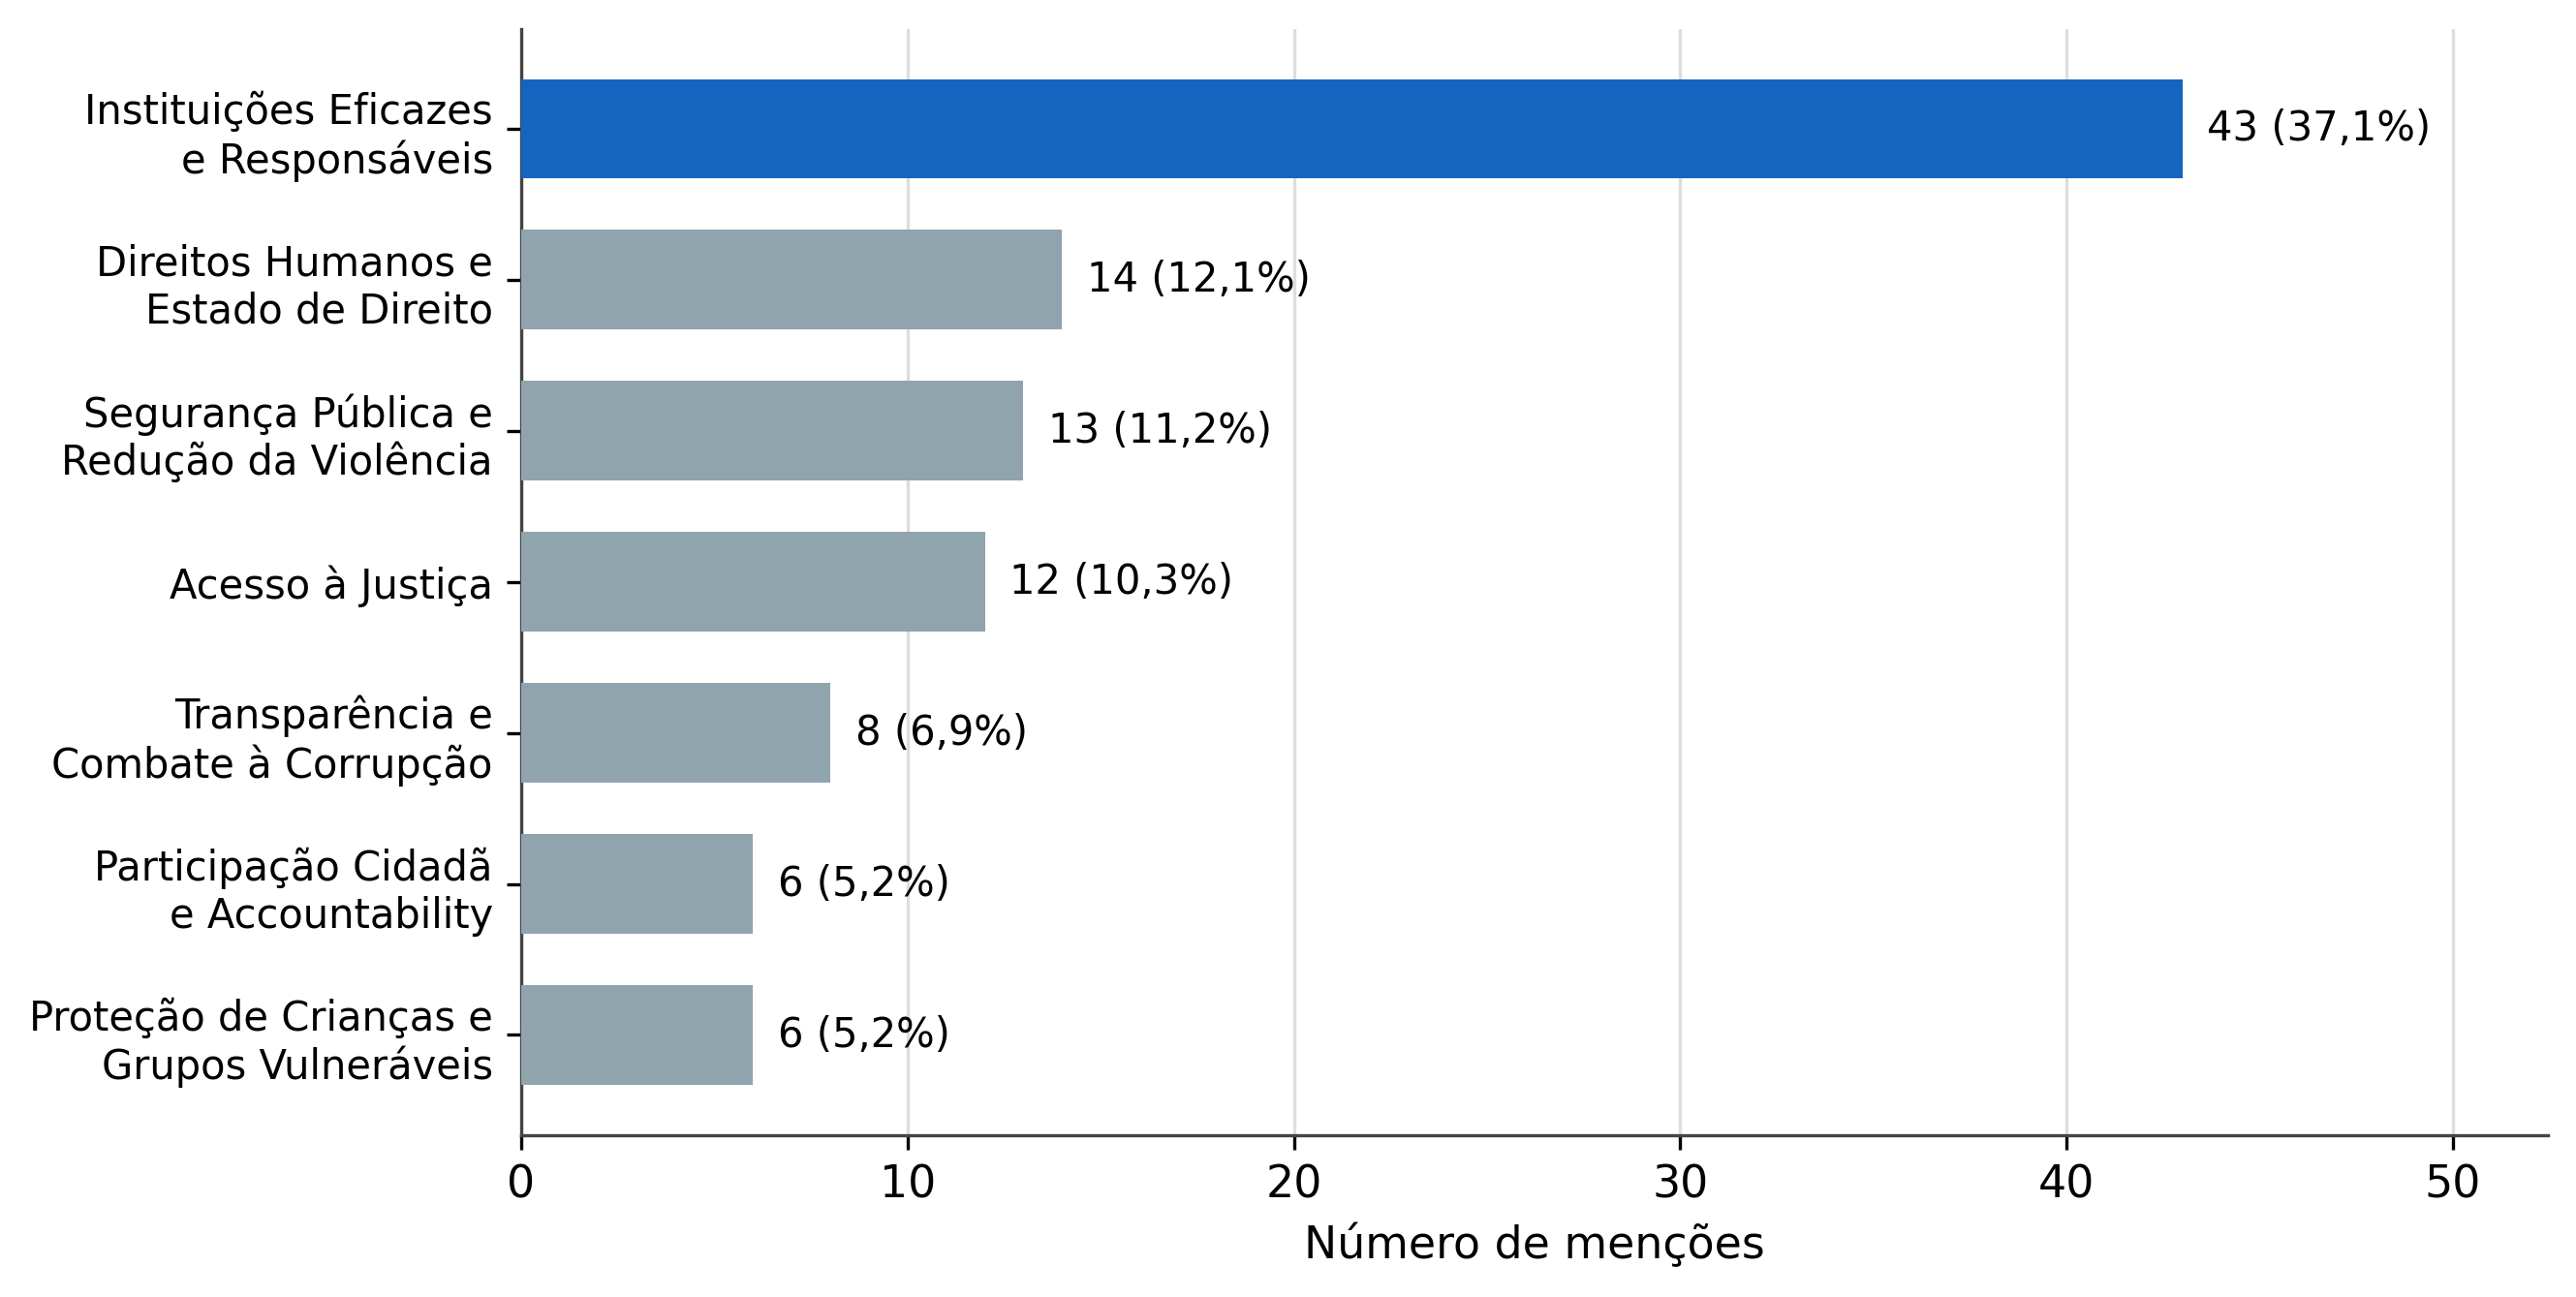
\includegraphics[width=0.90\textwidth]{figuras/problemas-dimensao-ods16}
    \legend{Fonte: Elaborado pelo autor (2026).}
\end{figure}

A dimensão \textit{Instituições Eficazes e Responsáveis} domina o conjunto de problemas (37,1\% das menções), evidenciando que a ineficiência administrativa é a raiz da maioria dos problemas identificados para o ODS 16 em Mossoró. Os principais problemas relatados nesta dimensão incluem: atendimento demorado e burocrático em secretarias municipais, insuficiência de pessoal, piora do atendimento com a migração para canais digitais e deficiências de gestão.

As demais dimensões reforçam esse quadro de fragilidade institucional. \textit{Direitos Humanos e Estado de Direito} registrou 14 menções (12,1\%), evidenciando violações em contextos de fiscalização e necessidade de capacitação. \textit{Segurança Pública e Redução da Violência} somou 13 menções (11,2\%), associadas à atuação insuficiente dos órgãos de segurança e à sensação de insegurança. \textit{Acesso à Justiça} (12 menções -- 10,3\%) relacionou-se à burocracia excessiva e a dificuldades de atendimento presencial. \textit{Transparência e Combate à Corrupção} (6,9\%), \textit{Participação Cidadã e Accountability} (5,2\%) e \textit{Proteção de Crianças e Grupos Vulneráveis} (5,2\%) completam o quadro de fragilidades identificadas.

\subsection{Dashboard ODS 16}
\label{subsec:dashboard-ods16}

A Figura~\ref{fig:dashboard-ods16} apresenta o dashboard web para o ODS 16, que permite exploração interativa dos 116 registros coletados.

\begin{figure}[h!]
    \centering
    \caption{Dashboard web -- ODS 16: Paz, Justiça e Instituições Eficazes em Mossoró-RN}
    \label{fig:dashboard-ods16}
    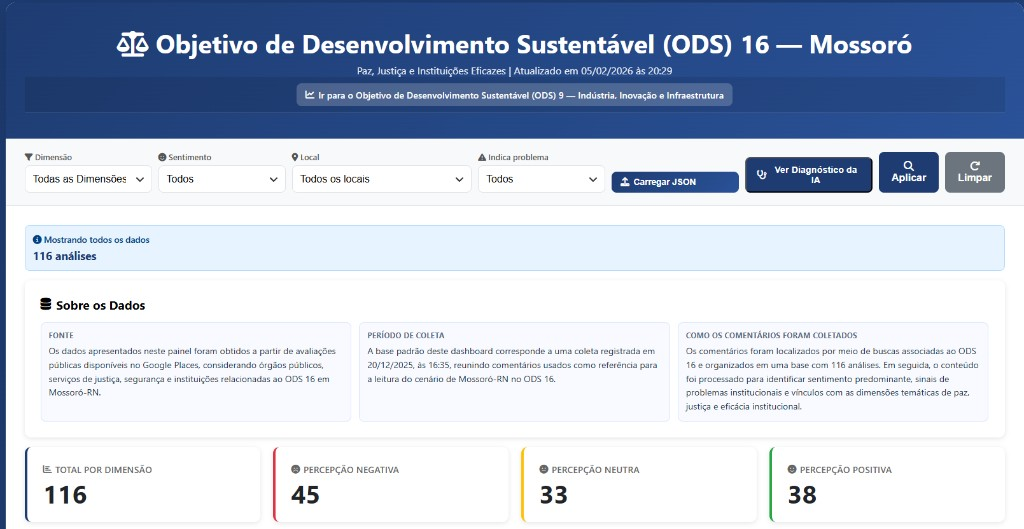
\includegraphics[width=0.95\textwidth]{figuras/dashboard-web-ods16}
    \legend{Fonte: Elaborado pelo autor (2025).}
\end{figure}

\section{Diagnósticos Gerados Automaticamente}
\label{sec:diagnosticos-automaticos}

O sistema gerou diagnósticos estruturados em linguagem natural para cada ODS, sintetizando os padrões identificados nas análises individuais. Cada diagnóstico é composto por seis blocos: diagnóstico geral do baixo desempenho, análise por dimensão, pontos críticos prioritários, impacto social e urbano, recomendações estratégicas e conclusão. Para o ODS 9, o diagnóstico identificou a degradação da infraestrutura física -- especialmente o Terminal Rodoviário -- como gargalo central, com impacto em cascata sobre o transporte público, a mobilidade urbana e a economia local. Para o ODS 16, o diagnóstico apontou a fragilidade institucional sistêmica como causa-raiz, amplificando problemas em segurança pública, acesso à justiça e direitos humanos.

A seguir, apresenta-se um trecho representativo do diagnóstico gerado para cada ODS, transcrito do campo \texttt{conclusao\_geral\_diagnostico} dos arquivos JSON de resultados. Para o ODS 9, o diagnóstico geral e o trecho da análise dimensional de infraestrutura ilustram a capacidade do sistema de articular os indicadores quantitativos com as evidências qualitativas extraídas das avaliações:

\begin{citacao}
A análise de 253 avaliações coletadas sobre Mossoró-RN revela que 144 análises (56,9\%) identificam problemas que contribuem diretamente para o baixo desempenho no ODS 9 (pontuação muito baixa: 0--39,99). A distribuição de sentimentos mostra predominância negativa: 103 análises negativas (40,7\%), 113 neutras (44,7\%) e apenas 37 positivas (14,6\%). Esta distribuição evidencia um cenário crítico de infraestrutura, inovação e desenvolvimento industrial na cidade. [...] Infraestrutura Resiliente e Moderna: os problemas mais frequentes incluem infraestrutura deteriorada, falta de manutenção, estacionamentos inadequados, banheiros em estado deplorável e necessidade urgente de reformas. A rodoviária de Mossoró é descrita como ``cenário pós-apocalíptico'', com estruturas abandonadas, sujas e em risco de colapso. Ruas precisam de reformas urgentes e há falta de serviços básicos em terminais e espaços públicos. (Diagnóstico gerado automaticamente pelo sistema, 2025)
\end{citacao}

Para o ODS 16, o trecho selecionado evidencia a identificação da fragilidade institucional como causa central do baixo desempenho:

\begin{citacao}
Mossoró-RN apresenta pontuação \textit{muito baixa} no ODS 16 (0--39,99) pautada por percepção pública amplamente crítica sobre a capacidade institucional e pelo registro significativo de análises que vinculam falhas institucionais à fragilização da paz e da justiça; das 116 análises, 54 (46,6\%) foram identificadas como contributivas para o baixo desempenho no ODS 16, com 43 menções explícitas a \textit{instituições eficazes} como problema central. [...] Instituições Eficazes e Responsáveis: esta é a dimensão mais citada (43 menções) e apresenta as falhas mais determinantes para o desempenho baixo: ineficiência no atendimento público, piora do serviço em migração para canais digitais, insuficiência de pessoal, deficiências de gestão em secretarias e falta de escalabilidade de práticas eficazes. As análises indicam baixa confiança institucional e fragilidade administrativa que comprometem implementação de políticas, execução de serviços essenciais e resposta a demandas cidadãs. (Diagnóstico gerado automaticamente pelo sistema, 2025)
\end{citacao}

Os trechos ilustram duas características relevantes da geração automatizada: a fidelidade aos números agregados da coleta, reproduzidos corretamente nos textos, e a incorporação de evidências textuais extraídas diretamente das avaliações dos cidadãos, como a descrição da rodoviária. Os diagnósticos gerados foram validados por comparação com os problemas identificados manualmente na literatura e em relatórios de organismos oficiais. A consistência entre os achados automatizados e as evidências conhecidas confirma a capacidade do sistema de produzir diagnósticos confiáveis a partir de dados não estruturados.

A Figura~\ref{fig:diagnostico-ods9} ilustra a página de diagnóstico textual do ODS 9, na qual o usuário pode consultar o diagnóstico geral e os diagnósticos por dimensão. A página organiza o texto produzido pela IA em uma interface de leitura própria, separando a exploração quantitativa do dashboard da análise qualitativa gerada automaticamente.

\begin{figure}[H]
    \centering
    \caption{Página web de diagnóstico automatizado -- ODS 9}
    \label{fig:diagnostico-ods9}
    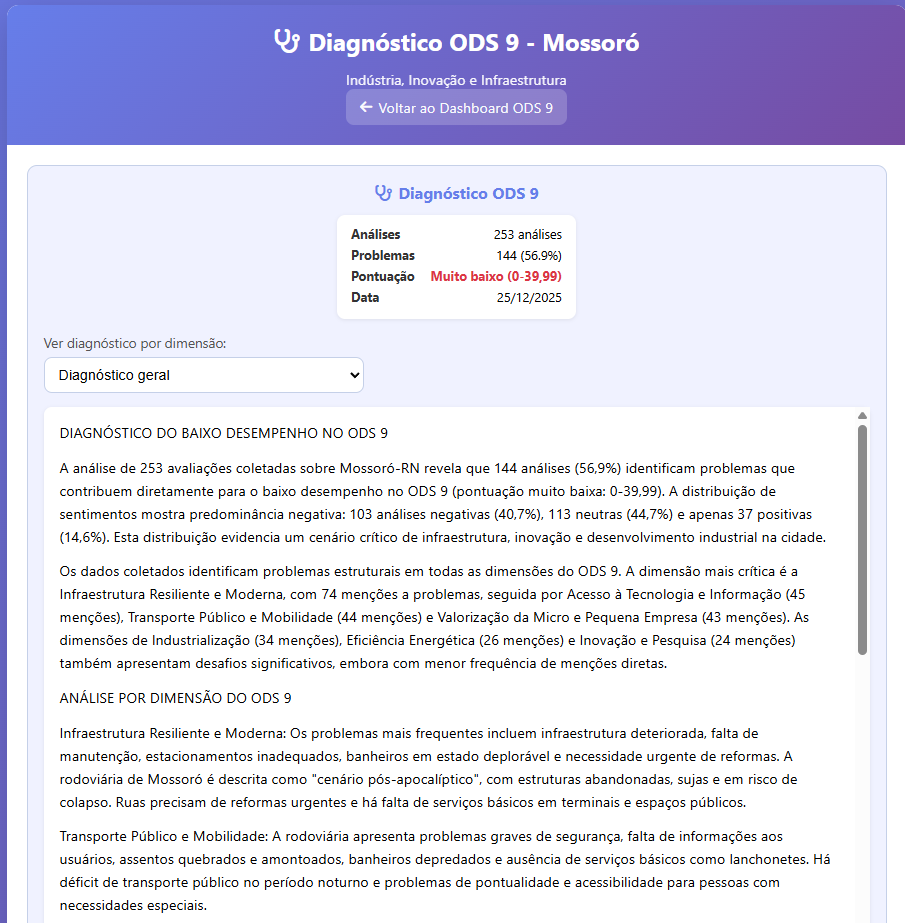
\includegraphics[width=0.70\textwidth]{figuras/diagnostico-web-ods9}
    \legend{Fonte: Elaborado pelo autor (2025).}
\end{figure}
\FloatBarrier
\section{Evidências de Generalização da Abordagem}
\label{sec:generalizacao-abordagem}

Embora o estudo de caso principal desta dissertação concentre-se em Mossoró-RN, com ênfase nos ODS 9 e 16, a implementação também foi avaliada quanto à sua capacidade de generalização para outros objetivos e municípios. Essa verificação foi realizada por meio da execução do motor de análise em diferentes combinações de ODS, cidade e conjunto de dimensões, mantendo a mesma lógica de coleta, filtragem, análise por aspecto, geração de JSON e produção de diagnóstico automatizado.

A generalização foi testada em dois níveis. No primeiro, os modelos específicos de ODS foram reaplicados em outras cidades (Natal-RN, Fortaleza-CE, João Pessoa-PB e Salvador-BA), mantendo a estrutura de análise definida para cada objetivo. No segundo, a versão genérica orientada por arquivos de configuração JSON foi executada sem alteração do código-fonte para os ODS 3 e 4, modificando apenas os parâmetros de entrada relativos ao ODS, à localidade, às dimensões e aos termos de busca. Os detalhes operacionais dessas execuções, incluindo os arquivos de configuração utilizados e os volumes coletados, são apresentados nas Seções~\ref{sec:generalizacao-multiplos-ods} e~\ref{sec:generalizacao-geografica}.

Essas execuções não substituem o estudo de caso aprofundado realizado em Mossoró-RN, mas demonstram que a arquitetura proposta não está rigidamente acoplada a um único município ou a um único ODS. A possibilidade de alterar o arquivo de configuração e reaplicar a pipeline a novos contextos constitui uma evidência técnica de escalabilidade. Assim, a abordagem pode ser replicada para outros municípios brasileiros, desde que existam avaliações públicas disponíveis na Google Places API e que as dimensões do ODS analisado sejam adequadamente parametrizadas.

É importante destacar que a generalização aqui apresentada é de natureza técnica e operacional. Ou seja, demonstra que o sistema executa a coleta, a filtragem, a análise e a geração de diagnósticos em diferentes contextos. A generalização substantiva dos achados -- isto é, a afirmação de que os mesmos problemas identificados em Mossoró ocorrem em outras cidades -- requer estudos comparativos adicionais, com validação local e análise das especificidades urbanas, institucionais e socioeconômicas de cada município.

\section{Correlações entre Dimensões e Padrões Transversais}
\label{sec:correlacoes}

A análise comparativa entre os dois ODS revelou padrões estruturais comuns que transcendem as especificidades de cada objetivo:

\begin{itemize}
    \item \textbf{Falta de manutenção preventiva}: tanto a infraestrutura física (ODS 9) quanto os serviços institucionais (ODS 16) degradam-se por ausência de manutenção e monitoramento contínuos;
    \item \textbf{Insuficiência de recursos humanos e financeiros}: ambos os ODS sofrem com quadros de pessoal reduzidos e orçamento insuficiente para atender a demanda;
    \item \textbf{Desconexão com necessidades cidadãs}: os serviços públicos analisados mostram baixa capacidade de resposta às demandas da população, evidenciada nas avaliações;
    \item \textbf{Concentração geográfica de problemas}: os estabelecimentos com maior número de avaliações negativas concentram-se no centro e em terminais de transporte, sugerindo prioridades claras de intervenção.
\end{itemize}

Para o ODS 16, a análise identificou uma cadeia causal entre as dimensões: instituições ineficazes amplificam barreiras ao acesso à justiça, que por sua vez contribuem para violações de direitos humanos e redução da participação cidadã, retroalimentando a fragilidade institucional.
